\section{Überlegungen für die Multilane-Szenarios}\sa{Einrückung und Linebreaks entfernen}
\label{sec:ueberlegungen-multilane}

Aufgrund zweier Fehler\footnote{siehe \url{https://github.com/LightJason/AgentSpeak/issues/47} und \url{https://github.com/LightJason/AgentSpeak/issues/50}} im Agenten-Framework, die bis zum Termin dieser Arbeit nicht behoben wurden, war es nicht möglich, auch belastende Tests für die Mehrspurszenarien durchzuführen.

Dennoch sind theoretische Überlegungen und in Teilen getestete praktische Vorarbeiten vorhanden, die in diesem Kapitel präsentiert werden sollen.



%%%%%%%%%%%%%%%%%%%%%%%%%%%%%%%%%%%%%%%%%%%%%%%%%%%%%%%%%%%
%	NEW SUBSECTION
%%%%%%%%%%%%%%%%%%%%%%%%%%%%%%%%%%%%%%%%%%%%%%%%%%%%%%%%%%%



\subsection{Veränderungen für die Mehrspurigkeit}\sa{keine leeren Kapitel}
\label{sec:multilane-change}


\subsubsection{Zustandsautomat}\sa{Linereaks und Einrückungen entfernen}

Für die Simulation mehrspuriger Fahrbahnen kann der ursprüngliche Zustandsautomat (\cref{figure:fsm-nasch}), der die Veränderung der Geschwindigkeit beinhaltet, unverändert bleiben.
Das Spurwechselverhalten wird in einem separaten Automaten abgebildet, siehe \cref{figure:fsm-pull}.

\begin{figure}[hptb]
 \centering
 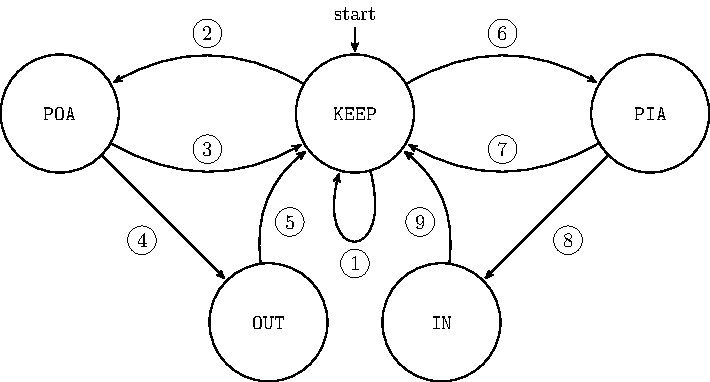
\includegraphics[width=0.9\textwidth]{fsm-pull}
 \caption[Zustandsautomat für das Spurverhalten]
 		{Zustandsautomat für das Agentenverhalten Spur halten/Spur wechseln}
 \label{figure:fsm-pull}
\end{figure}

Der Startzustand des Automaten, \texttt{KEEP} (keep lane/Spur halten), steht für das Verhalten, die aktuelle Spur beizubehalten.

Aus diesem Zustand heraus sind die Zustände \texttt{POA} (Pull-out attempt/Ausscherversuch) und \texttt{PIA} (Pull-in attempt/Einscherversuch) zu erreichen.
Ein Ausscherversuch kann z.B. unternommen werden, wenn das Fahrzeug auf ein anderes Fahrzeug aufläuft.
\\
Ist keiner der Spurwechselversuche möglich, kann der Zustand \texttt{KEEP} über eine Schleife auch wieder selbst erreicht werden.

Sowohl aus \texttt{POA}, als auch aus \texttt{PIA} ist ein Übergang zurück zu \texttt{KEEP} möglich.
Dieser Pfad wird genommen, wenn der jeweilige Versuch abgebrochen werden muss.
\\
Für den Ausscherversuch könnte dies beispielsweise aufgrund von seitlichem Verkehr auf der Überholspur der Fall sein.

Sind die Voraussetzungen für einen sichern Spurwechsel gegeben, erfolgt jeweils der Übergang in die Zustände \texttt{OUT} (pull out/Ausscheren) bzw. \texttt{IN} (pull in/Einscheren) und von dort aus wieder in den \texttt{KEEP}-Zustand.

Auch hier entspricht ein Zeitschritt der Simulation einem Zyklus vom Startzustand ausgehend bis zur Rückkehr dorthin.



\subsubsection{Agentenverhalten}\sa{Einrücken und Linebreaks entferenen}
\label{sec:agentplan-multilane}

Die Veränderungen im Grundplan des Agentenverhaltens sind minimal. 
Es müssen lediglich zwei Ziele für das Ausscheren (Pull-out) und das Einscheren (Pull-in) hinzugefügt werden.
Dies wird durch die jeweiligen Pläne ergänzt.
Für das komplette Agentenscript siehe \cref{lst:multi-lane}.

Der Aufruf des jeweiligen Plans und das Abarbeiten der Bedingungen entspricht dabei dem Spurwechselversuch.
Die Ausführung wird aus dem Agentenplan an die Simulationssoftware weiter geleitet.

\begin{minipage}[hptb]{0.95\textwidth}
\begin{lstlisting}[style=asl, 
                   keywords={!pullout,!pullin}, 
                   keywords={[2]vehicle/pullout,vehicle/pullin}, 
                   keywords={[3]}, 
                   caption={Auszug aus Agentenscript: multi lane-Version},
                   label={lst:multilane-auszug}]      
!cruise.

// --- start all other plans ---
+!cruise <-
    !accelerate;
    !decelerate;
    !linger;
    !pullout
    !pullin
    !cruise
.

// --- pull-out, change lane to overtake ---
+!pullout
    : // --- Bedingungen gekuerzt ---
    <- vehicle/pullout
.

// --- pull-in, change lane after overtake is finished ---
+!pullin
    : // --- Bedingungen gekuerzt ---
    <- vehicle/pullin
.\end{lstlisting}
\end{minipage}

\paragraph*{Der \texttt{pullout}-Plan}\sa{Überschrift wissenschaftliche benennen, Einrückung und Linebreaks entfernen}
\hfill \\
Der Plan für das Ausscheren ist mit insgesamt fünf Bedingungen versehen.

\begin{enumerate}
	\itemsep0em
	\item Befindet sich das Fahrzeug nicht auf der am weitesten linken Fahrspur?
	\item Ist in der aktuellen Spur Verkehr voraus?
	\item Ist der Verkehr in der Spur, in die gewechselt werden soll, nicht näher?
	\item Befindet sich kein Verkehr direkt links neben dem Fahrzeug in der Nachbarspur?
	\item Ist der rückwärtige Verkehr auf der Zielspur nicht zu nah?
\end{enumerate}

Die erste Bedingung ist zwingend notwendig, da sonst keine Spur zum hineinwechseln vorhanden wäre.
Die Auslösung eines Kollisionsereignisses wäre in der Simulation die Folge.
\\
Die zweite Bedingung macht den Ausschervorgang erst nötig. 
Wäre die aktuelle Spur nicht blockiert, könnte auf ihr weitergefahren werden.
\\
Ein Spurwechsel ist nur sinnvoll, wenn auf der zukünftigen Spur mindestens genauso viel Raum nach vorn ist, wie auf der aktuellen. 
Dem trägt Bedingung 3 Rechnung.
\\
Durch die Unterteilung des Sichtfeldes in vier Sektoren, siehe \cref{sec:unterteilung-sichtfeld}, wurde die vierte Bedingung notwendig.
\\
Um den nachfolgenden Verkehr nicht zu behindern, ist die fünfte Regel zu beachten.

Durch die Fehler im Framework ist die gleichzeitige Auswertung aller Bedingungen unmöglich.
\\
Bei keiner der Bedingungen ist es möglich, diese wegzulassen oder mit einer anderen zusammenzufassen, ohne dass unerwünschtes Verhalten auftritt.

Würden zum Beispiel die Bedingungen 2 und 3 zusammengefasst und nur auf vorwärtigen Verkehr (in beiden Spuren) geprüft, so würde dies zwar der Bedingung \enquote{nicht schlechter} für die Überholspur genügen, aber jedes überholende Fahrzeug würde zum Auslösen dieser Bedingung führen.

Eine Auslagerung der Bedingungen 1 und 2 in den \texttt{cruise}-Plan erscheint auch nicht sinnvoll, weil diese Kontrolle einen Zeitschritt vor Ausführung des Planes geschehen würde.
Der Spurwechsel selbst würde dann mit noch einem Zeitschritt Verzögerung ausgeführt werden.
\\
Außerdem könnte es zu Inkonsistenzen bzgl. der aktuellen Fahrspur kommen.
So könnte der Agent in einem Zeitschritt den Spurwechsel ausführen, gleichzeitig aber nochmals den \texttt{pullout}-Plan anstoßen.
Dort würde dann nicht wieder geprüft, in welcher Spur sich der Agent befindet.
Somit würde ein weiteres Ausschermanöver ausgeführt, ohne dass eine Zielspur vorhanden wäre.

Ein \enquote{Workaround} wäre, Verkehr auf der Zielspur generell auszuschließen.
Dieser Plan würde aber nicht optimal arbeiten. 



\paragraph*{Der \texttt{pullin}-Plan}\sa{Linbreak und Einrückungen entfernen} 
\hfill \\
Im Plan für das Einscheren sind vier Bedingungen zu beachten.

\begin{enumerate}
	\itemsep0em
	\item Befindet sich das Fahrzeug nicht auf der am weitesten rechten Fahrspur?
	\item Ist in der Spur, in die gewechselt werden soll, genügend Abstand nach vorn?
	\item Befindet sich kein Verkehr direkt rechts neben dem Fahrzeug in der Nachbarspur?
	\item Ist der rückwärtige Verkehr auf der Zielspur ausreichend weit entfernt?
\end{enumerate}

Wie auch beim Ausscheren muss sich in Orientierungsrichtung mindestens eine weitere Spur befinden, da es sonst zum Auslösen des Kollisionsereignisses durch die Simulationssoftware kommt.
Hierfür sorgt die erste Bedingung.

Bedingung 2 sorgt dafür, dass das Fahrzeug selbst einige Zeit freie Fahrt auf der Zielspur hat.
Die Bedingungen 3 und 4 bewirken, dass kein anderer Verkehr behindert wird. 

Auch die Ausführung dieses Planes ist durch die Fehler im Agenten-Framework betroffen. Allerdings gibt es einen \enquote{Workaround}, der aber kein optimales Verhalten liefern kann.
\\
Das kollisionsfreie Wiedereinordnen kann garantiert werden, wenn sich keinerlei Verkehr im Sichtfeld des Fahrzeuges befindet.
Dies ist jedoch bei Simulationen mit vielen Fahrzeugen nahezu unmöglich.



%%%%%%%%%%%%%%%%%%%%%%%%%%%%%%%%%%%%%%%%%%%%%%%%%%%%%%%%%%%
%	NEW SUBSECTION
%%%%%%%%%%%%%%%%%%%%%%%%%%%%%%%%%%%%%%%%%%%%%%%%%%%%%%%%%%%



\subsection{Testläufe des Mehrspurmodells}
\label{test-multilane}

Da die erdachte Logik nicht funktionierte, wurde überlegt, mit welchen Alternativen bzw. Workarounds dennoch ein Teil des Verhaltes getestet werden könnte.
Die o.a. Alternativen wurden jew. in einem separeten Plan umgesetzt.
Belastende Tests konnten mit diesen allerdings nicht durchgeführt werden.
\\
Bereits bei drei Fahrzeugen im System kam es zu Situationen, bei denen das Einscheren ausblieb.

\paragraph*{Spurwechsel/Überholmanöver}\sa{keine leeren Kapitel}
\hfill \\
\begin{figure}[hptb]
  \centering 
   \subfigure[Spurnutzung, überholendes Fahrzeug]{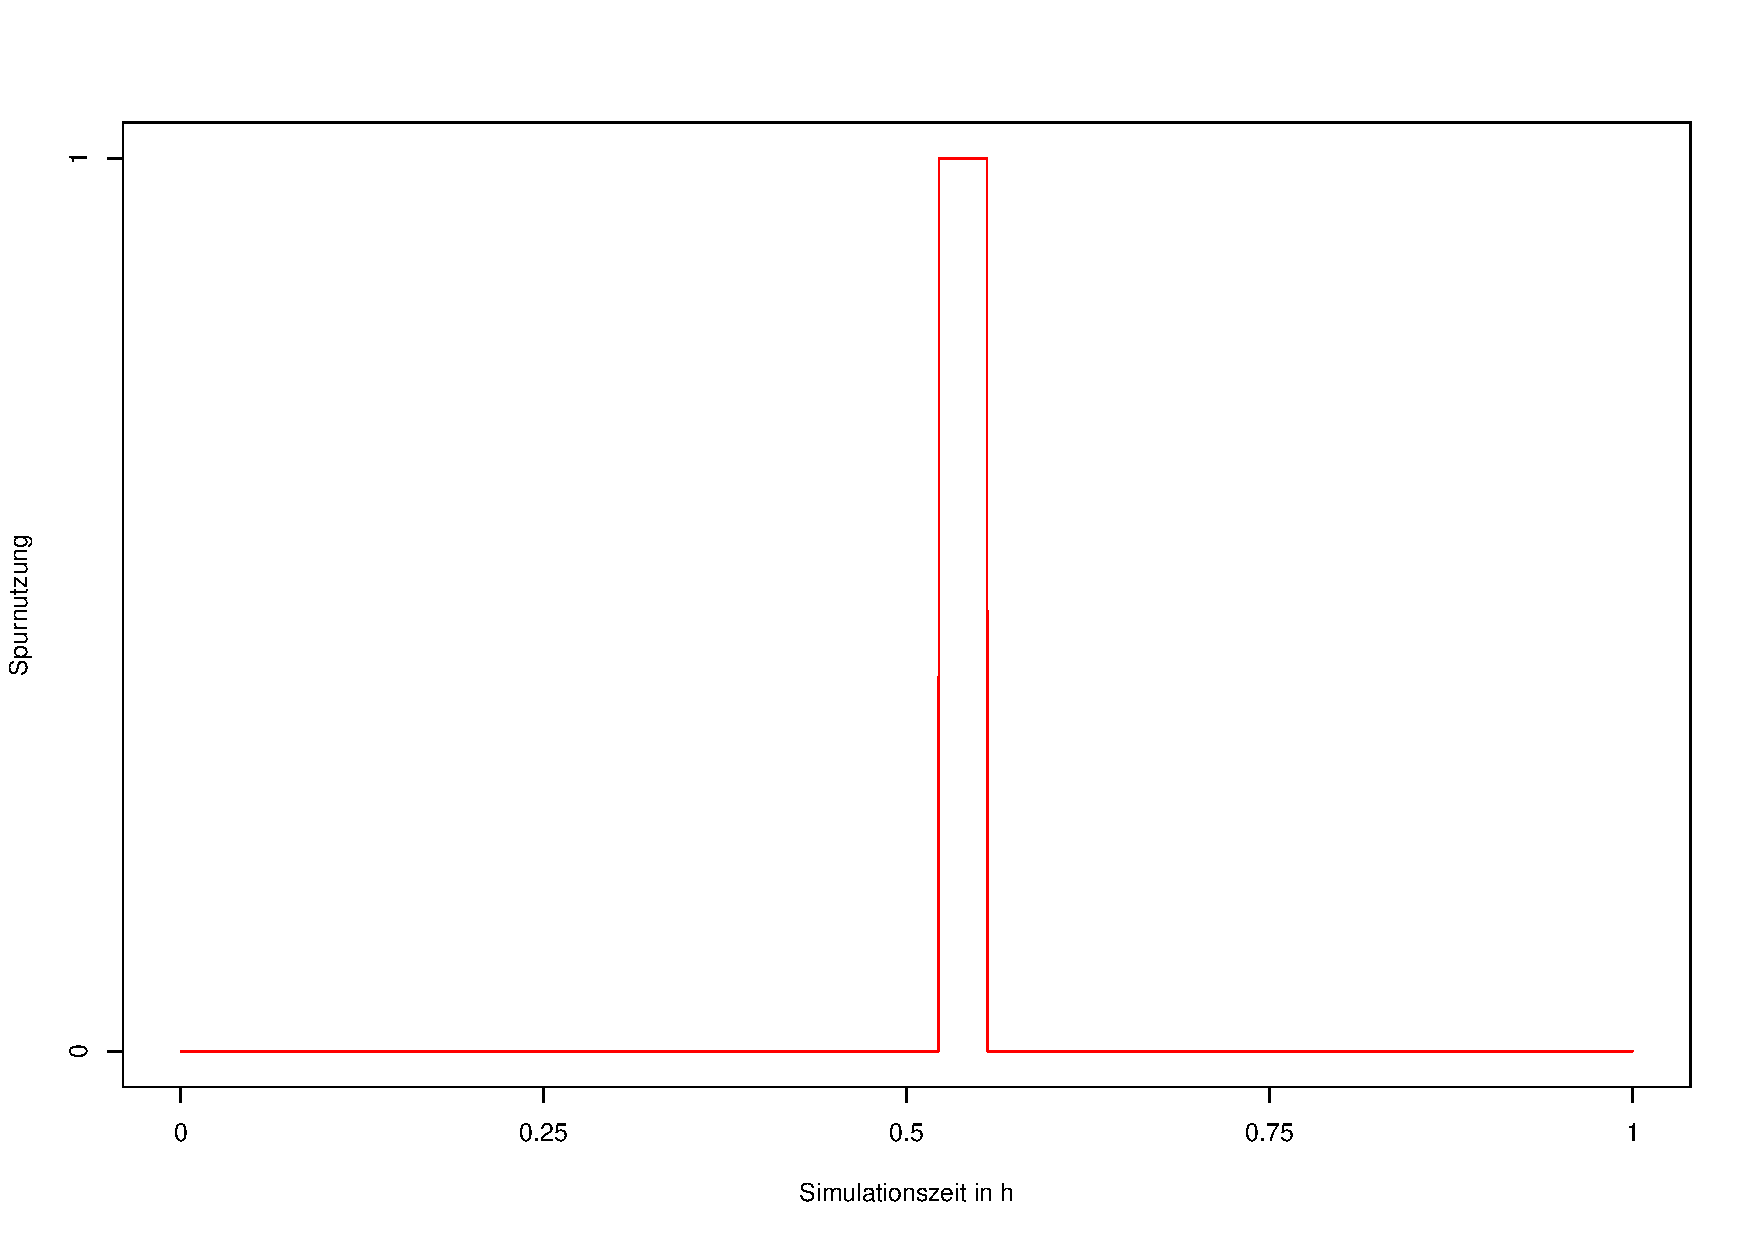
\includegraphics[width=0.45\textwidth]{multi-overtake-lane}\label{figure:multi-overtake-lane}}\qquad 
   \subfigure[Geschwindigkeit, beide Fahrzeuge]{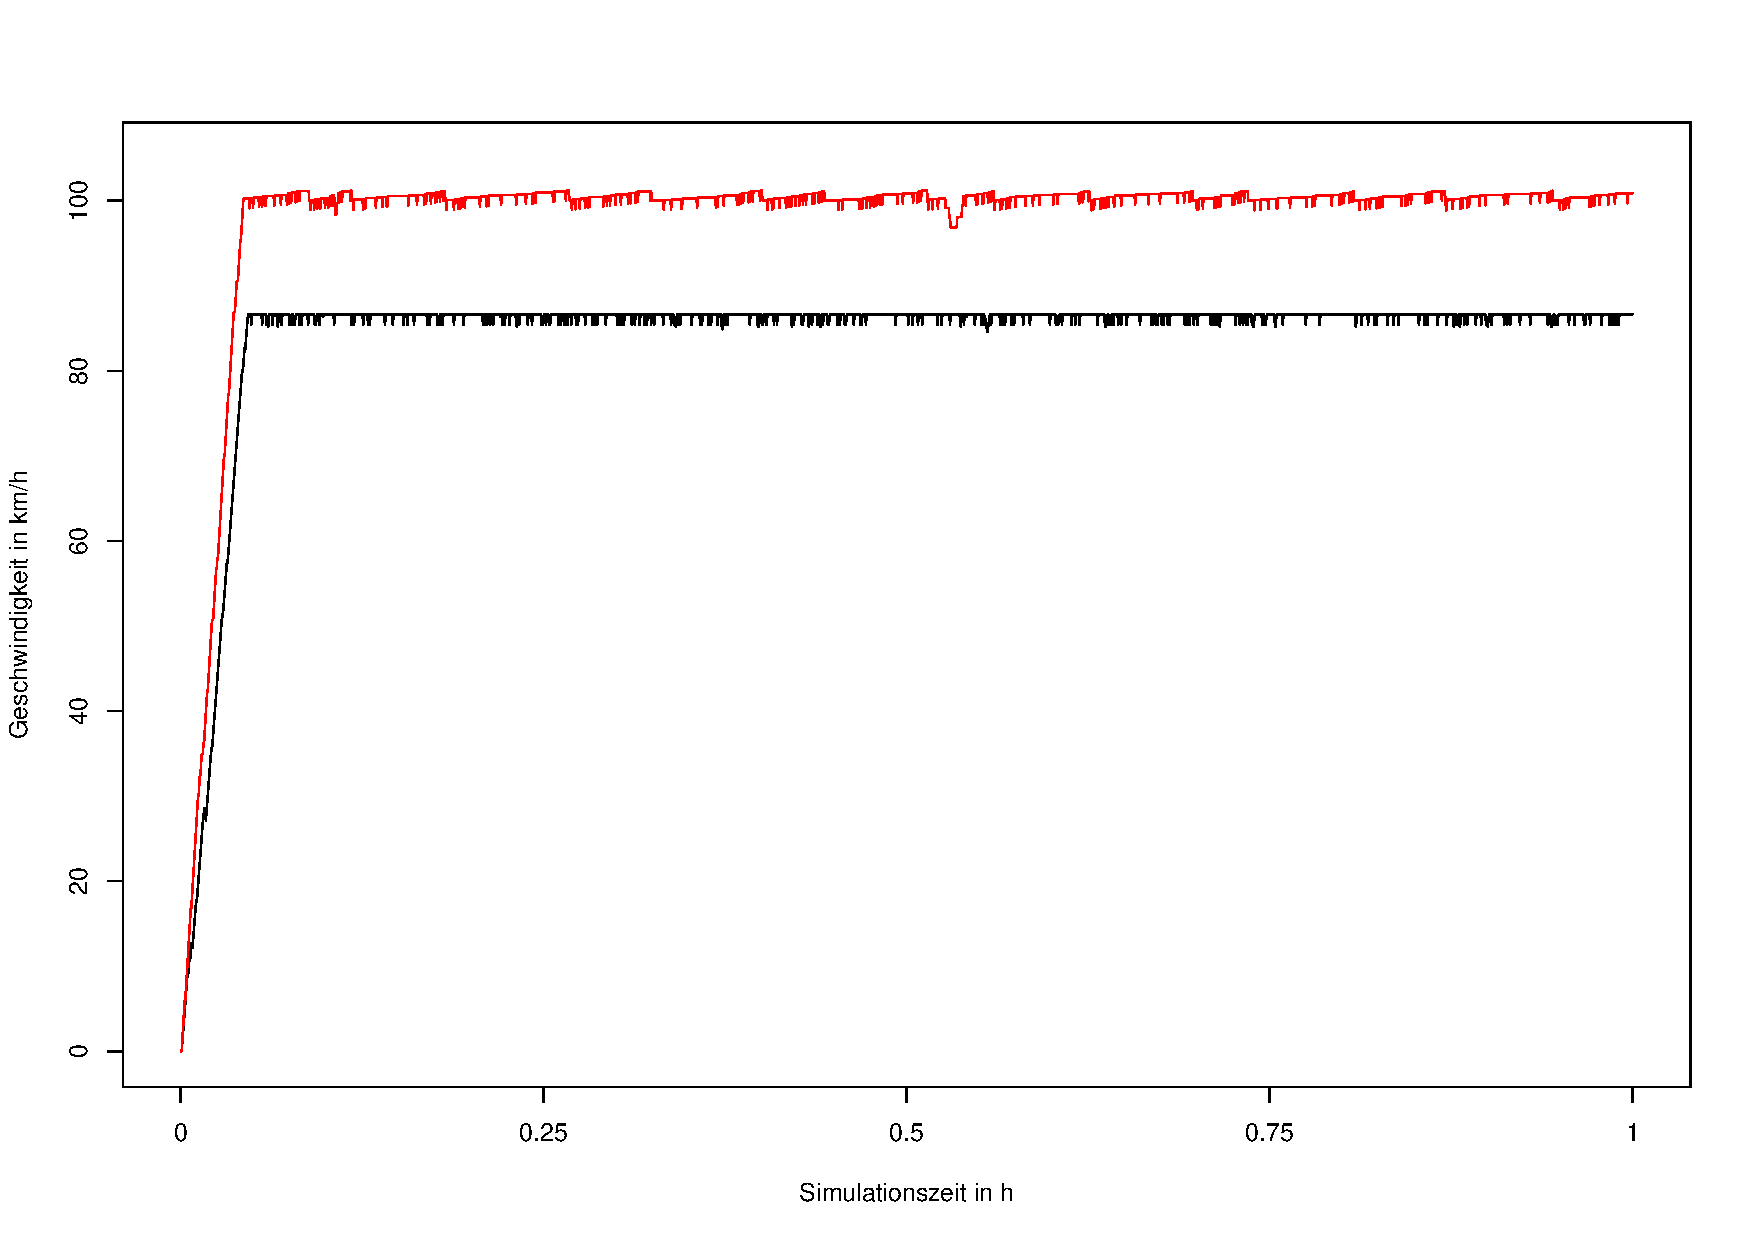
\includegraphics[width=0.45\textwidth]{multi-overtake-speed}\label{figure:multi-overtake-speed}} \\ 
   \subfigure[Positionen, beide Fahrzeuge]{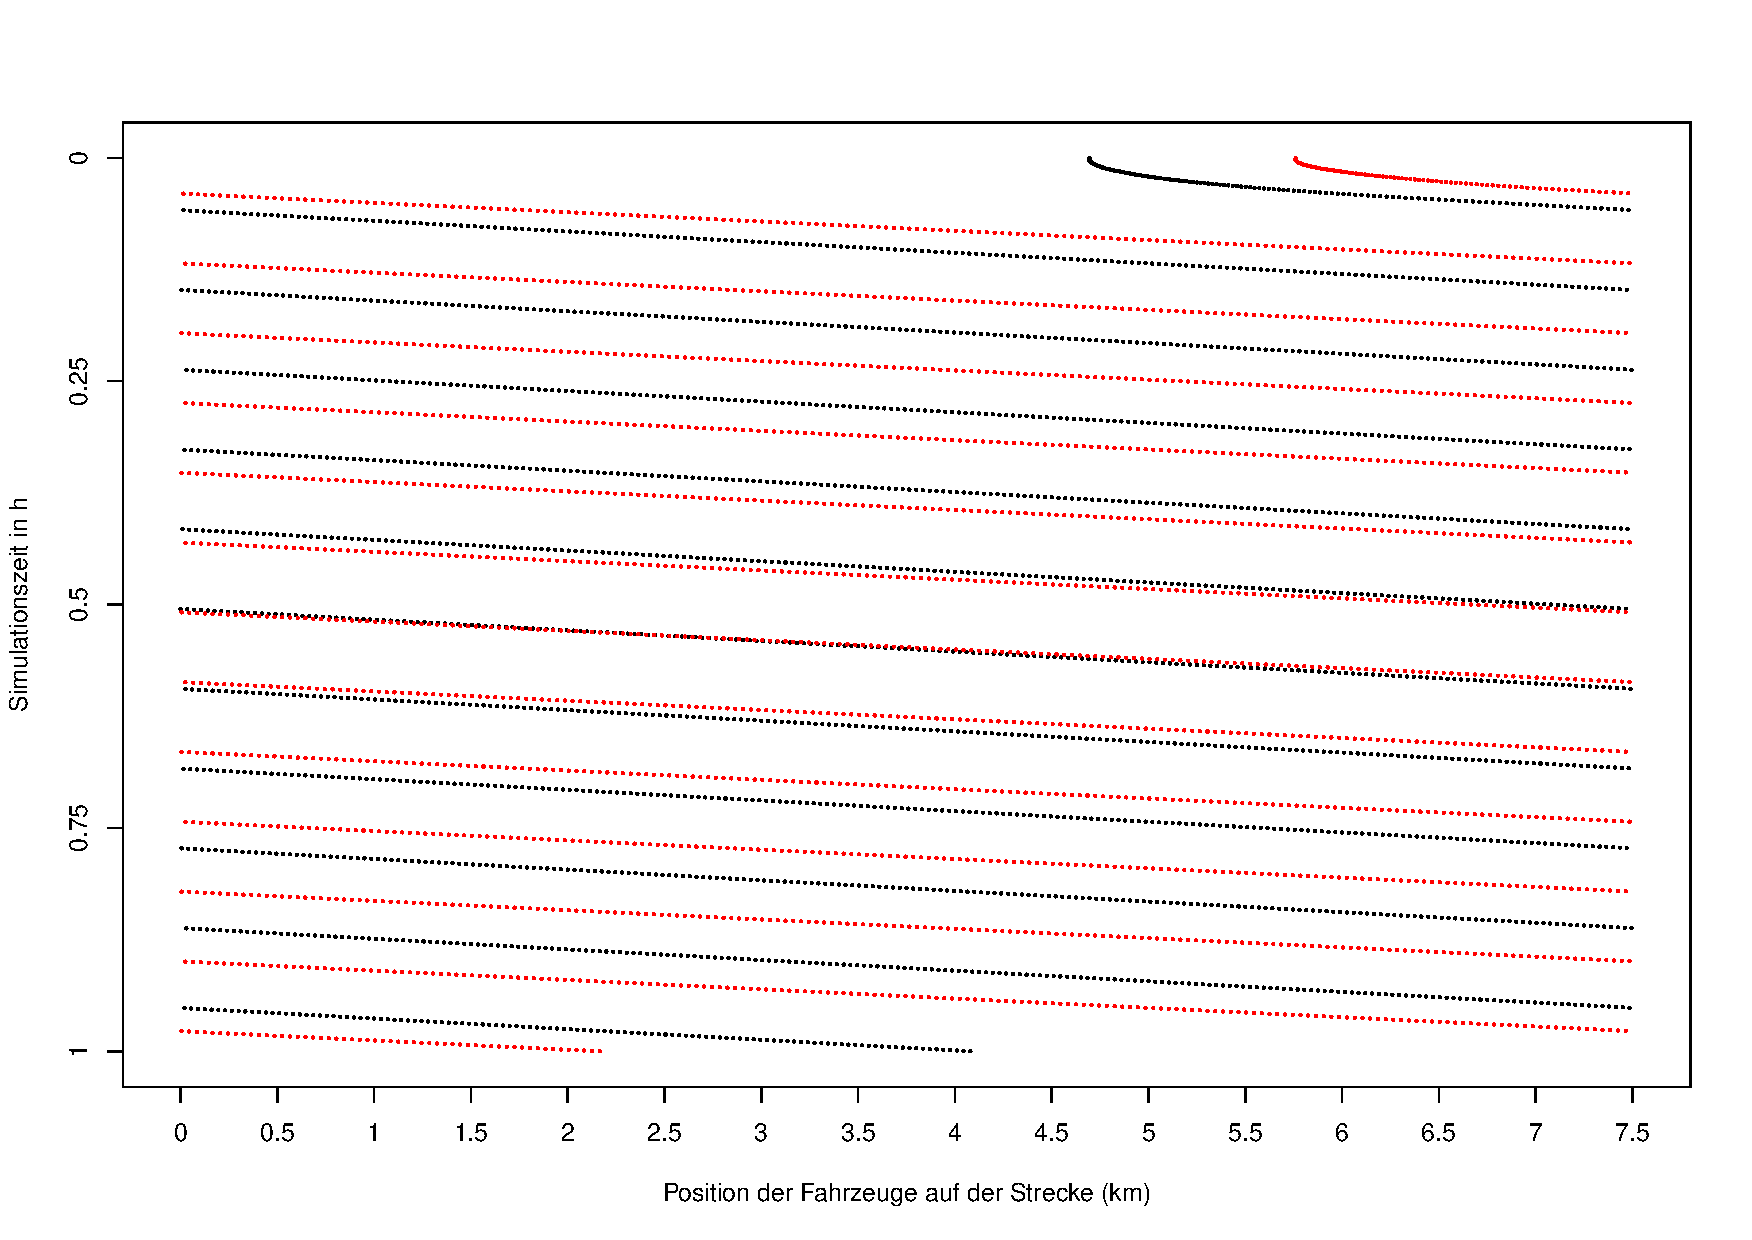
\includegraphics[width=1\textwidth]{multi-overtake-position}\label{figure:multi-overtake-position}}
  \caption{Überholen im Multilane-Szenario} 
  \label{figure:multi-overtake}
\end{figure}



%%%%%%%%%%%%%%%%%%%%%%%%%%%%%%%%%%%%%%%%%%%%%%%%%%%%%%%%%%%
%	NEW SUBSECTION
%%%%%%%%%%%%%%%%%%%%%%%%%%%%%%%%%%%%%%%%%%%%%%%%%%%%%%%%%%%



\subsection{Zufälligkeit des Aus- und Einscherens}\sa{Linebreaks und Einrückungen entfernen}
\label{sec:additional-extensions}



\subsubsection{Zufälligkeit des Aus- und Einscherens}
\label{sec:pullout-pullin}

Um unterschiedliche Verhaltensweisen beim Überholen im Autobahnverkehr abbilden zu können, benötigt man einen Mechanismus, Wahrscheinlichkeiten für jew. eine der Handlungen zu generieren.

Dieses wurde z.B. in \cite{dat-ba} anhand des \enquote{Social-Force-Vehicle-Modells} versucht. 
Der dort erarbeitete Ansatz scheint jedoch das gewünschte Verhalten übermäßig zu bevorteilen.

Für den Anreiz zum Spurwechsel nach links (Pull-out) oder rechts (Pull-in) genügt im Zweispurfall die Berechnung der jeweiligen Wahrscheinlichkeit.
Die Wahrscheinlichkeit, die Spur zu halten, wäre jeweils die Gegenwahrscheinlichkeit.
\\
Für Szenarien mit mehr als zwei Spuren ist eine Exklusivität (XOR) der beiden Ereignisse zu gewährleisten.
Hier könnte die Wahl auf die Alternative mit der größeren Wahrscheinlichkeit fallen bei exakter Gleichheit würde es Sinn machen, aufgrund des zu überholenden Verkehrs und des Verbotes des rechts Überholens, den Spurwechsel nach links zu präferieren.

\paragraph*{Wahrscheinlichkeitsfunktion} 
\hfill \\
Für eine Bestimmung von Wahrscheinlichkeiten für diesen Zweck erscheint die logistische Funktion  
\begin{center}
$ f(x) = \frac{1}{1 + e^{-x}} $ 
\end{center}
siehe \cite{logistic-function}, eine Sigmoid-Funktion (auch S- oder Schwanenhalsfunktion), ein geeigneter Kandidat. 
Sie ist für alle Zahlen in $ \mathbb{R} $ definiert und ihr Wertebereich liegt zwischen 0 und 1.

\begin{figure}[hptb]
  \centering
    \subfigure[Grundform]{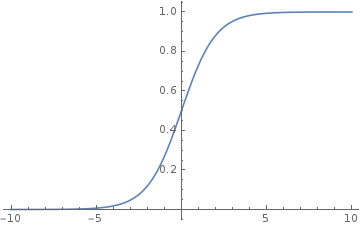
\includegraphics[width=0.45\textwidth]{kurve-logistic-10-10}\label{figure:kurve-logistic-10-10}} \qquad 
    \subfigure[gestreckte Form]{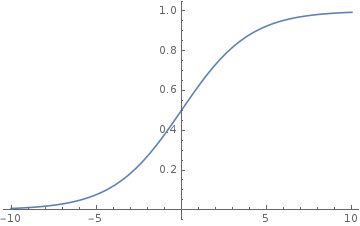
\includegraphics[width=0.45\textwidth]{kurve-logistic-streched-10-10}\label{figure:kurve-logistic-streched-10-10}}
  \caption[Kurvenbeispiele der logistischen Funktion]
          {Kurvenbeispiele logistischer Funktionen im identischen Intervall}
  \label{figure:kurve-logistic}
\end{figure}

\noindent
Die Grundfunktion (\cref{figure:kurve-logistic-10-10}) steigt im Intervall $ [-5; 5] $ ziemlich rasch von nahe 0 auf nahe 1.
Dies kann durch Streckung der Funktion etwas abgemildert werden.
So verläuft z.B. 
\begin{center}
$ f(x) = \frac{1}{1 + e^{-\frac{1}{2}x}} $ 
\end{center}
weniger steil (\cref{figure:kurve-logistic-streched-10-10}) und hat den für diesen Zweck sinnvoll nutzbaren Intervall $ [-10; 10 ] $.
Für Werte außerhalb dieses Intervalles ergibt sich jeweils entweder eine kleine von Null, bzw. große von Eins verschiedene Wahrscheinlichkeit.

\paragraph*{Wahrscheinlichkeit des Ausscherens (Pull-out)} 
\hfill \\
Für das Ausscheren wurden die folgende Zusammenhänge, bezogen auf ein vorausfahrendes Fahrzeug, erkannt:
\begin{itemize}
    \itemsep0em
    \item Abstand $ \searrow $  $ \Longrightarrow $ Ausscherwunsch $ \nearrow $ (und umgekehrt)
    \item relative Geschwindigkeit $ \nearrow $ $ \Longrightarrow $ Ausscherwunsch $ \nearrow $ (und umgekehrt)
\end{itemize}

Es galt sinnvolle Werte zu finden und diese auf den o.g. Intervall zu normieren.

Für den Abstand $ s $ wurde die Grenze der Zone der Nahortientierung/Handlung, siehe \cref{sec:sichtweite} - 110 m - und ein Punkt, an dem nach Möglichkeit spätestens ein Überholvorgang eingeleitet sein sollte - 50 m - gewählt.
\\
Dies führt zu der Funktion
\begin{center}
$ f(s) = -\frac{s}{3} + \frac{80}{3} $
\end{center}
Somit ergibt sich für die Überholwahrscheinlichkeit in Abhängigkeit vom Abstand zum vorausfahrenden Fahrzeug $ p_{po}(s) $ die Funktion
\begin{center}
$ p_{po}(s) = \frac{1}{1 + e^{-\frac{1}{2}f(s)}} $
\end{center}

\noindent
Für die relative Geschwindigkeit $ v_{rel} $ wurden die Grenzen bei 0 und 25 km/h festgelegt.
Ab 0 km/h bzw. darunter ist kein Überholen mehr nötig.
Für die obere Grenze wurde das Verhalten auf Landstraßen\sa{Referenz anstatt Fußnote}\footnote{siehe \url{https://www.adac.de/_mmm/pdf/fachdossier_ueberholen_auf_landstra\%C3\%9Fen_68414.pdf}, S. 27, abgerufen am 07. März 2018.}
%, siehe \cite[S. 27]{ueberholgeschwindigkeit}, 
auf den Autobahnverkehr übertragen.
\\
Dies führt zu der Funktion 
\begin{center}
$ f(v_{rel}) = \frac{4 v_{rel}}{5} - 10 $
\end{center}
Für die Überholwahrscheinlichkeit in Abhängigkeit von der relativen Geschwindigkeit zum vorausfahrenden Fahrzeug $ p_{po}(v_{rel}) $ ergibt sich
\begin{center}
$ p_{po}(v_{rel}) = \frac{1}{1 + e^{-\frac{1}{2}f(v_{rel})}} $
\end{center}

\noindent
Eine Kombination der beiden Gleichungen und Normierung auf den Intervall $ [0; 1] $
\begin{center}
$ p_{po} = \frac{1}{2}(p_{po}(s) + p_{po}(v_{rel})) = \frac{1}{2}p_{po}(s) + \frac{1}{2}p_{po}(v_{rel}) $
\end{center}
liefert die Wahrscheinlichkeit für das Ausscheren $ p_{po} $.
Hier wären die beiden Wahrscheinlichkeiten gleich gewichtet (Faktor $ \frac{1}{2} $). Eine unterschiedliche Gewichtung kann durch Faktoren, welche in Summe 1 ergeben müssen, herbeigeführt werden.

Es ergibt sich eine Funktionskurve mit der Ausbildung von drei erkennbaren Plateaus um die Wahrscheinlichkeitswerte 0, 0,5 und 1, siehe \cref{figure:kurve-ueberholwahrscheinlichkeit}.
%Die Darstellung erfolgt in den Intervallen  $ [0; 1] $ für die Wahrscheinlichkeit, $ [ 40; 120 ] $ für den Abstand und $ [ -5; 30 ] $ für die relative Geschwindigkeit.

\begin{figure}[hptb]
 \centering
 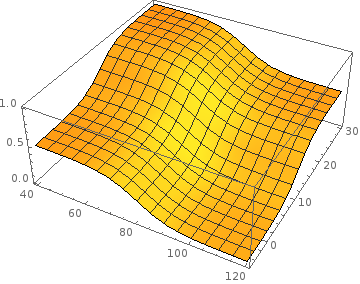
\includegraphics[width=0.5\textwidth]{kurve-ueberholwahrscheinlichkeit}
 \caption[Funktionskurve für die Ausscherwahrscheinlichkeit]
 		 {Plateaubildung der Funktionskurve der Ausscherwahrscheinlichkeit}
 		 {\footnotesize(für $ p_{po} \in [0; 1] $, $ s \in [ 40; 120 ] $, $ v_{rel} \in [ -5; 30 ] $)}
 \label{figure:kurve-ueberholwahrscheinlichkeit}
\end{figure} 


\paragraph*{Wahrscheinlichkeit des Einscherens (Pull-in)} 
\hfill \\
Eine ähnliche Herangehensweise ist für das Einscheren möglich.
Hier müssten allerdings sowohl der vorausfahrende Verkehr $ T_{f} $, als auch der rückwärtige Verkehr $ T_{b} $ beachtet werden. 
Aufgrund der fehlenden Möglichkeit eines Tests, wird hier nur das Konzept umrissen.

\begin{itemize}
    \itemsep0em
    \item Abstand $ T_{f} $ $ \nearrow $ $ \Longrightarrow $ Einscherdrang $ \nearrow $ (und umgekehrt)
    \item relative Geschwindigkeit $ T_{f} $ $ \searrow $ $ \Longrightarrow $ Einscherdrang $ \nearrow $ (und umgekehrt)
    \item Abstand $ T_{b} $ $ \nearrow $ $ \Longrightarrow $ Einscherdrang $ \nearrow $ (und umgekehrt)
    \item relative Geschwindigkeit $ T_{b} $ $ \nearrow $ $ \Longrightarrow $ Einscherdrang $ \nearrow $ (und umgekehrt)
\end{itemize}

Beim Zusammenfassen der entstehenden einzelnen Wahrscheinlichkeiten kann ebenfalls wieder über Faktoren eine individuelle Gewichtung vorgenommen werden.



\subsubsection{Dosiertes Abbremsen}

In den zugrunde liegenden Tests wurde das Abbremsen mit maximal möglicher Intensität ausgeführt.
Denkbar wäre auch hier die Verwendung der logistischen Funktion, um die Bremsstärke zu dosieren.
Ähnlich wie beim Ausscheren scheinen Abstand und relative Geschwindigkeit als zu beachtende Größen sinnvoll.



\subsubsection{Vermeidung des Rechts-Überholens}

Um Fahrzeuge in der Simulation vom Überholen auf der rechten Seite abzuhalten ist nur eine einfache Bedingung im \texttt{decelerate}-Plan notwendig, siehe \cref{lst:multilane-rechts}.

\begin{minipage}[hptb]{0.95\textwidth}
\begin{lstlisting}[style=asl, 
                   keywords={Lane,CurrentLane}, 
                   keywords={[2]}, 
                   keywords={[3]}, 
                   caption={Auszug aus Agentenscript: Überholverbot rechts},
                   label={lst:multilane-rechts}]      
!decelerate
// --- gekuerzt ---
    : >>( view/vehicle( _, data( _, static( lane( Lane ), cell( Cell ), speed( Speed ), distance( Dist ), direction( Dir ) ) ) ), 
            bool/equal( generic/type/tostring( Dir ), "forward[]" ) 
            && math/floor(Lane) > CurrentLane
            && Speed < CurrentSpeed
            && Dist < 1.5*CurrentSpeed
        ) <-
        CurrentSpeed > 80 ? vehicle/decelerate(0.9) : vehicle/decelerate(0.5);
.\end{lstlisting}
\end{minipage}

Je weiter links eine Fahrspur ist, desto größer ist ihre Id.
Befindet sich also im Sichtfeld von Fahrzeug A ein Fahrzeug B auf einer Fahrspur mit größerer Id, so wird von Fahrzeug A ein Bremsmanöver eingeleitet.
\\
Weitere Einschränkungen ergeben sich durch die Hinzunahme einer Geschwindigkeits- und einer Abstandskomponente.

Außerdem ist eine Erweiterung im \texttt{accelerate}-Plan erforderlich, dass eine Beschleunigung auch bei vorausfahrendem Verkehr auf Spuren mit größerer Id ausbleiben kann.

Das Verhalten, was diese Bedingung auslöst, konnte getestet werden, indem ein langsameres Fahrzeug auf der Überholspur fuhr und das schnellere auf der Normalspur aufschloss.
Das schnellere Fahrzeug bremste ab und passte sich der Geschwindigkeit des langsameren Fahrzeugs an.
